\documentclass[12pt]{article}
\usepackage{sbc-template} 
\usepackage{graphicx,url}
\usepackage{url}
\usepackage[brazil]{babel} 
\usepackage[utf8]{inputenc} 
\usepackage[T1]{fontenc}
\usepackage[normalem]{ulem}
\usepackage[hidelinks]{hyperref}

\usepackage[square,authoryear]{natbib}
\usepackage{amssymb} 
\usepackage{mathalfa} 
\usepackage{algorithm} 
\usepackage{algpseudocode} 
\usepackage[table]{xcolor}
\usepackage{array}
\usepackage{titlesec}
\usepackage{mdframed}
\usepackage{listings}

\usepackage{amsmath} 
\usepackage{booktabs}

\urlstyle{same}

\newcolumntype{L}[1]{>{\raggedright\let\newline\\\arraybackslash\hspace{0pt}}m{#1}}
\newcolumntype{C}[1]{>{\centering\let\newline\\\arraybackslash\hspace{0pt}}m{#1}}
\newcolumntype{R}[1]{>{\raggedleft\let\newline\\\arraybackslash\hspace{0pt}}m{#1}}

\newcommand\Tstrut{\rule{0pt}{2.6ex}} 
\newcommand\Bstrut{\rule[-0.9ex]{0pt}{0pt}} 
\newcommand{\scell}[2][c]{\begin{tabular}[#1]{@{}c@{}}#2\end{tabular}}

\usepackage[nolist,nohyperlinks]{acronym}

\title{Trabalho Prático II - Análise Empírica e Otimização para o Caixeiro Viajante}

\author{Larissa Oliveira Aguiar\inst{1}}


\address{Universidade Federal de Minas Gerais - UFMG
\email{larissaaguiar@ufmg.br}
}



\begin{document} 
	
	\maketitle
	
	\begin{resumo} 
        Este relatório descreve a implementação e avaliação experimental de algoritmos para o Problema do Caixeiro Viajante (Traveling Salesperson Problem – TSP). Foram estudados três métodos: Branch-and-Bound (BB), Twice-around-the-tree e algoritmo de Christofides. Na implementação do BB, foram investigadas diferentes estratégias de inicialização de solução viável (warm starts), tais como,ingenua, vizinho mais próximo, fecho convexo, Twice-around-the-tree e Christofides.  A avaliação experimental considera o tempo de execução, o consumo de memória, os nós expandidos e podados, a qualidade das soluções e o impacto das características geométricas das instâncias no desempenho dos algoritmos. Também são investigados os custos das principais subrotinas e o comportamento empírico dos métodos em função do tamanho das instâncias. Os resultados permitem discutir as vantagens e limitações das estratégias aproximativas e exatas.
	\end{resumo}
	 Repositório: https://github.com/larisaguiar/tp2-caixeiro-viajante
     
	\section{Introdução}
	\label{sec_introducao}	
    Problemas de otimização combinatória estão presentes em diversas áreas da computação e da engenharia, especialmente em situações que exigem encontrar a melhor solução entre um conjunto muito grande de possibilidades. Entre esses problemas, destaca-se o Problema do Caixeiro Viajante (Traveling Salesperson Problem – TSP), que consiste em determinar uma rota de menor custo que percorra um conjunto de cidades, visitando cada uma exatamente uma vez e retornando à cidade de origem. Apesar de sua definição simples, o TSP apresenta elevada complexidade computacional, sendo classificado como um problema NP-difícil. Dessa forma, encontrar soluções ótimas torna-se progressivamente mais custoso à medida que o número de cidades aumenta.

O estudo do TSP é relevante não apenas por suas aplicações em problemas de roteamento, logística e planejamento de trajetórias, mas também por permitir investigar diferentes estratégias de projeto e análise de algoritmos. Enquanto métodos exatos buscam garantir a obtenção da solução ótima, métodos aproximativos procuram produzir soluções de boa qualidade em tempo computacional reduzido. Essa diferença evidencia um dos principais desafios da otimização combinatória: equilibrar qualidade da solução, tempo de execução e consumo de memória. Assim, a comparação entre essas abordagens permite compreender em quais condições cada estratégia apresenta melhores resultados e quais limitações podem comprometer sua utilização.

Nesse contexto, este trabalho aborda a implementação e a avaliação de algoritmos para resolução do Problema do Caixeiro Viajante, considerando tanto métodos exatos quanto aproximativos. São estudados o algoritmo Branch-and-Bound, como abordagem exata, e os algoritmos Twice-around-the-tree e Christofides, como abordagens aproximativas. No Branch-and-Bound, a eficiência da busca depende diretamente da qualidade dos limites inferiores utilizados para descartar caminhos que não podem produzir uma solução melhor que a melhor rota conhecida. Além disso, a qualidade da solução inicial, utilizada como limite superior, pode influenciar significativamente a quantidade de nós explorados durante a execução. Portanto, a escolha da estratégia de busca e dos métodos de inicialização constitui parte importante do problema investigado.

O objetivo geral deste trabalho é implementar, auditar e avaliar experimentalmente algoritmos exatos e aproximativos para o TSP, investigando seu desempenho e a influência das características das instâncias sobre a qualidade das soluções e o custo computacional. Como objetivos específicos, busca-se implementar os algoritmos Twice-around-the-tree e Christofides; desenvolver e analisar uma solução Branch-and-Bound; comparar cinco estratégias de inicialização para o algoritmo exato — rota trivial, vizinho mais próximo, inserção de vértices a partir do fecho convexo, Twice-around-the-tree e Christofides —; investigar o impacto dessas estratégias na quantidade de nós expandidos e podados; e avaliar o tempo de execução, o consumo de memória e a qualidade das soluções obtidas.

Adicionalmente, o trabalho contempla a auditoria e o aprimoramento da implementação do Branch-and-Bound. A versão inicial utiliza uma estratégia de busca Best-First, baseada em uma fila de prioridade que seleciona os nós com menores limites inferiores. A partir da análise de seu comportamento, investiga-se a utilização de uma estratégia de busca em profundidade (Depth-First Search – DFS), considerando principalmente o impacto das estruturas de dados sobre o consumo de memória. Também são analisadas as subrotinas de maior custo computacional e a relação entre o tamanho das instâncias e o tempo de execução dos algoritmos. Por fim, são extraídas características geométricas e estruturais das instâncias para investigar possíveis relações entre essas propriedades, a qualidade das soluções aproximativas e o esforço exigido pela busca exata.

As contribuições deste trabalho consistem na comparação experimental de diferentes algoritmos para o TSP, na análise do impacto de estratégias de inicialização sobre o Branch-and-Bound, na auditoria de alternativas de exploração da árvore de busca e na investigação da influência de características das instâncias sobre o desempenho dos métodos avaliados. Dessa maneira, pretende-se não apenas comparar os resultados obtidos, mas também compreender os fatores que explicam as diferenças de desempenho entre as abordagens estudadas.

O restante deste trabalho está organizado da seguinte forma: a Seção 2 apresenta os fundamentos teóricos do Problema do Caixeiro Viajante e dos algoritmos utilizados. A Seção 3 descreve os detalhes de implementação, as estruturas de dados e as decisões tomadas durante a auditoria e o aprimoramento dos algoritmos. A Seção 4 apresenta a metodologia experimental, incluindo as instâncias utilizadas, as métricas coletadas e os procedimentos de análise. A Seção 5 discute os resultados obtidos, considerando o desempenho computacional, a qualidade das soluções, as estratégias de inicialização e a influência das características das instâncias. Por fim, a Seção 6 apresenta as conclusões e possíveis direções para trabalhos futuros.
	
	
	


\section{Fundamentação Teórica}

Esta seção apresenta os principais conceitos teóricos relacionados ao
Problema do Caixeiro Viajante (TSP) e aos algoritmos utilizados neste
trabalho. São abordadas a definição formal do problema, sua complexidade
computacional, os métodos exatos e aproximativos considerados, as
estratégias de construção de soluções iniciais e os conceitos necessários
para a avaliação experimental dos algoritmos.

\subsection{Problema do Caixeiro Viajante}

O Problema do Caixeiro Viajante (\textit{Traveling Salesperson Problem}
-- TSP) é um problema clássico de otimização combinatória. Seu objetivo
consiste em encontrar um caminho de menor custo que visite todos os vértices
de um grafo exatamente uma vez e retorne ao vértice de origem.

Formalmente, o problema pode ser representado por um grafo completo
ponderado $G=(V,E)$, em que $V$ representa o conjunto de vértices e
$E$ representa o conjunto de arestas. Cada aresta $(i,j)\in E$ possui
um custo $c_{ij}$, que representa a distância ou o custo de deslocamento
entre os vértices $i$ e $j$.

Uma propriedade importante para o estudo dos algoritmos aproximativos
é a desigualdade triangular. Uma função de distância satisfaz essa
propriedade quando, para quaisquer vértices $i$, $j$ e $k$, vale:

\begin{equation}
d(i,k)\leq d(i,j)+d(j,k).
\label{eq:desigualdade-triangular}
\end{equation}

Essa propriedade estabelece que o deslocamento direto entre dois
vértices não pode ser mais custoso do que realizar o percurso passando
por um terceiro vértice. Ela é uma condição importante para as garantias
clássicas de aproximação dos algoritmos Twice-around-the-tree e
Christofides.

\subsection{Complexidade Computacional}

O TSP pertence à classe dos problemas NP-difíceis, o que significa que
não é conhecido um algoritmo de tempo polinomial capaz de encontrar uma
solução ótima para todas as instâncias do problema. O número de possíveis
caminhos cresce  com a quantidade de vértices. Os algoritmos exatos procuram garantir a obtenção da solução ótima, mas podem apresentar elevado custo computacional. Em contrapartida, algoritmos
aproximativos priorizam a eficiência, aceitando soluções que podem não
ser ótimas, mas que possuem garantias teóricas de qualidade sob
determinadas condições.

\subsection{ Branch-and-Bound}

O Branch-and-Bound é uma técnica de otimização utilizada para resolver
problemas combinatórios por meio da exploração  de um espaço
de soluções. Seu funcionamento combina duas operações principais:
ramificação (\textit{branching}) e poda (\textit{bounding}).

A ramificação consiste em dividir o problema em subproblemas menores.
No contexto do TSP, cada nó da árvore de busca representa um caminho
parcial, construído pela seleção sucessiva de vértices ainda não
visitados.

A poda utiliza limites inferiores para identificar caminhos que não
poderão produzir uma solução melhor do que a melhor solução completa
conhecida. Essa solução conhecida fornece um limite superior
(\textit{upper bound}), enquanto o limite inferior (\textit{lower bound})
estima o menor custo que ainda pode ser alcançado a partir de determinado
caminho parcial.

Se o limite inferior de um nó for maior ou igual ao limite superior
atual, o nó pode ser descartado sem comprometer a obtenção da solução
ótima. 

A eficiência do Branch-and-Bound depende diretamente da qualidade
desses limites. Limites inferiores mais próximos do custo ótimo permitem
descartar mais subproblemas, enquanto limites superiores menores tornam
a condição de poda mais restritiva.

\subsubsection{Estratégias de Exploração da Árvore de Busca}

A ordem de exploração dos nós influencia o comportamento do
Branch-and-Bound. Entre as estratégias possíveis, destacam-se a busca
em largura, a busca em profundidade e a busca pelo melhor limite.

Na estratégia Best-First Search, os nós são armazenados em uma fila
de prioridade, geralmente implementada por meio de uma estrutura de
heap. A prioridade é atribuída ao limite inferior, de modo que o nó
com menor estimativa de custo seja explorado primeiro.

Na busca em profundidade (\textit{Depth-First Search}, DFS), a
exploração segue um caminho até que não seja mais possível avançar
ou que uma condição de poda seja satisfeita. Em seguida, o algoritmo
retorna a um nível anterior da árvore e explora outra alternativa.
Essa estratégia pode ser implementada utilizando uma pilha.

A escolha entre essas estratégias envolve um compromisso entre ordem
de exploração e consumo de memória. Enquanto a Best-First mantém uma
fronteira de nós ordenada por prioridade, a DFS tende a manter uma
quantidade menor de nós pendentes durante a exploração. Entretanto,
a eficiência de ambas também depende da qualidade dos limites
utilizados e da estrutura do espaço de busca.

\subsection{Algoritmos Aproximativos para o TSP}

Algoritmos aproximativos buscam encontrar soluções de boa qualidade
sem necessariamente explorar todo o espaço de possibilidades. Para
problemas de otimização combinatória, esses algoritmos são especialmente
relevantes quando a obtenção da solução ótima exige tempo computacional
elevado.

No caso do TSP métrico, isto é, quando os custos satisfazem a desigualdade
triangular, existem algoritmos com garantias teóricas sobre a qualidade
da solução produzida.

\subsubsection{Twice-around-the-tree}

O algoritmo Twice-around-the-tree é uma abordagem aproximativa baseada
na construção de uma árvore geradora mínima (\textit{Minimum Spanning
Tree} -- MST). Uma árvore geradora mínima conecta todos os vértices de
um grafo com o menor custo total possível, sem formar ciclos.

O algoritmo pode ser descrito em quatro etapas:

\begin{enumerate}
    \item Construir uma árvore geradora mínima do grafo.
    \item Duplicar todas as arestas da árvore, formando um multigrafo
    no qual todos os vértices possuem grau par.
    \item Encontrar um circuito Euleriano, que percorre cada aresta
    do multigrafo exatamente uma vez.
    \item Remover as visitas repetidas aos vértices, realizando atalhos
    para obter um ciclo Hamiltoniano.
\end{enumerate}

A duplicação das arestas garante que o grafo resultante seja conexo
e possua todos os vértices com grau par, condição  para a existência de um circuito Euleriano em um grafo
conexo.



\subsubsection{Algoritmo de Christofides}

O algoritmo de Christofides é outro método aproximativo para o TSP
métrico. Assim como o Twice-around-the-tree, utiliza uma árvore
geradora mínima, mas incorpora uma etapa adicional de emparelhamento
de vértices para conseguir  uma garantia de aproximação.

Seu funcionamento pode ser dividido nas seguintes etapas:

\begin{enumerate}
    \item Construir uma árvore geradora mínima do grafo.
    \item Identificar os vértices que possuem grau ímpar na árvore.
    \item Encontrar um emparelhamento perfeito de custo mínimo entre
    os vértices de grau ímpar.
    \item Combinar as arestas da árvore com as arestas do emparelhamento.
    \item Encontrar um circuito Euleriano no multigrafo resultante.
    \item Remover as visitas repetidas aos vértices por meio de atalhos,
    obtendo um ciclo Hamiltoniano.
\end{enumerate}

O emparelhamento perfeito conecta os vértices de grau ímpar em pares,
tornando todos os graus do multigrafo resultante pares. Como o número
de vértices de grau ímpar é sempre par, esse emparelhamento pode ser
construído.




\subsection{Estratégias de Construção de Soluções Iniciais}

Na Branch-and-Bound, uma solução completa encontrada antes ou durante
a exploração da árvore de busca estabelece um limite superior para
o problema. Quanto menor o custo dessa solução inicial, maior pode
ser a capacidade de poda do algoritmo.

As estratégias de inicialização,  denominadas \textit{warm
starts}, permitem fornecer uma rota inicial viável ao algoritmo.
Neste trabalho, são consideradas cinco estratégias.

A primeira estratégia consiste em construir uma rota trivial, na qual os vértices são visitados na mesma ordem em que aparecem na representação da instância. Essa abordagem não considera as distâncias entre os vértices durante a construção da rota, utilizando apenas a ordem original dos dados para gerar uma solução inicial.

A segunda estratégia é o algoritmo do vizinho mais próximo
(\textit{Nearest Neighbor}), que inicia em um vértice e seleciona,
a cada etapa, o vértice não visitado mais próximo da posição atual.
O procedimento continua até que todos os vértices tenham sido
visitados, retornando então à origem.

A terceira estratégia utiliza o fecho convexo (\textit{Convex Hull})
dos pontos. Inicialmente, são identificados os vértices pertencentes
ao contorno convexo da distribuição espacial. Os demais vértices
são inseridos  na rota, escolhendo-se uma posição
de inserção que produza o menor acréscimo de custo.

As duas estratégias restantes utilizam os algoritmos aproximativos
apresentados anteriormente: Twice-around-the-tree e Christofides.
As rotas produzidas por esses métodos podem ser utilizadas diretamente
como soluções iniciais do Branch-and-Bound.

\subsection{Avaliação Experimental e Características das Instâncias}

A avaliação de algoritmos de otimização não deve considerar apenas
o custo da solução encontrada. Também é necessário analisar os
recursos computacionais consumidos durante a execução e compreender
como as características das instâncias influenciam o desempenho.

Neste trabalho, são consideradas métricas como tempo de execução,
consumo de memória, quantidade de nós expandidos e quantidade de nós
podados. 	
	
	
\section{Implementação e Auditoria dos Algoritmos}

Esta seção apresenta os detalhes de implementação dos algoritmos
utilizados na resolução do trabalho prático. São descritas
as estruturas de dados adotadas, as estratégias de exploração da árvore
de busca, os métodos de construção de soluções aproximativas e as
estratégias de inicialização utilizadas no Branch-and-Bound. Além disso,  são discutidas as decisões tomadas durante a auditoria e o aprimoramento das implementações.

\subsection{Organização da Implementação}

A implementação foi desenvolvida em Python, utilizando estruturas
de dados e bibliotecas científicas para manipulação das instâncias,
cálculo de distâncias e execução dos algoritmos.

As instâncias são representadas por matrizes de distância, nas quais
a posição $(i,j)$ armazena o custo de deslocamento entre os vértices
$i$ e $j$. Essa representação permite consultar os custos das arestas
durante a construção das rotas e a exploração dos caminhos parciais.

A organização modular do projeto separa os algoritmos exatos,
os algoritmos aproximativos, as estratégias de inicialização,
a extração de características das instâncias e os procedimentos
de análise experimental. Essa separação facilita a manutenção,
a validação e a comparação dos métodos implementados.

\subsection{Implementação do Branch-and-Bound}

O algoritmo Branch-and-Bound foi implementado para explorar
sistematicamente os caminhos possíveis do TSP, utilizando limites
inferiores para realizar podas e uma solução completa conhecida
como limite superior.

Cada nó da árvore de busca armazena informações sobre o caminho
parcial construído, o custo acumulado, o limite inferior estimado
e os vértices já visitados. A identificação dos vértices visitados
permite verificar quais alternativas ainda podem ser adicionadas
ao caminho.

O custo acumulado corresponde à soma das arestas já selecionadas.
O limite inferior estima o menor custo que pode ser alcançado
considerando as decisões já tomadas e as conexões ainda necessárias
para completar o ciclo Hamiltoniano.

A cada expansão, são gerados novos caminhos pela inclusão de
vértices ainda não visitados. Os nós cujo limite inferior é maior
ou igual ao custo da melhor solução completa conhecida são
descartados, pois não podem produzir uma solução melhor.



\subsubsection{Estratégias de Exploração}

Na implementação inicial, foi utilizada a estratégia Best-First
Search, na qual os nós são armazenados em uma fila de prioridade.
A prioridade é determinada pelo limite inferior, permitindo
explorar primeiro os caminhos com menores estimativas de custo.

Essa abordagem favorece a exploração de caminhos potencialmente
promissores, mas exige a manutenção de uma fronteira de busca
ordenada. Conforme novos nós são gerados, a estrutura pode crescer
significativamente, aumentando o consumo de memória.

Durante a auditoria, também foi considerada a estratégia de busca
em profundidade (Depth-First Search -- DFS). Nessa abordagem,
os nós pendentes são armazenados em uma pilha, e a exploração
avança por um caminho antes de retornar para investigar outras
alternativas.

A adoção da DFS busca reduzir a quantidade de nós mantidos
simultaneamente na estrutura de busca. Para favorecer a exploração
de caminhos promissores, os sucessores podem ser ordenados de
acordo com seus limites inferiores antes de serem inseridos na
pilha.

A escolha da estratégia deve considerar o compromisso entre
ordem de exploração, capacidade de poda e consumo de memória.
Independentemente da estratégia utilizada, a garantia de
otimalidade depende da validade do limite inferior e da conclusão
da busca sem interrupções.



\subsection{Estratégias de Inicialização do Branch-and-Bound}

Foram consideradas cinco estratégias de inicialização para produzir uma solução viável inicial, utilizada como limite superior do Branch-and-Bound.

\begin{enumerate}
    \item \textbf{Cold Start:} utiliza uma caminho sequencial, visitando os vértices na ordem
    de representação da instância.

    \item \textbf{Nearest Neighbor:} seleciona o vértice não visitado mais próximo do vértice atual.

    \item \textbf{Convex Hull:} constrói inicialmente uma rota com os vértices do fecho convexo
    e insere os vértices internos nas posições de menor acréscimo de custo.

    \item \textbf{Twice-around-the-tree:} utiliza o caminho produzido pelo algoritmo aproximativo
    de mesmo nome.

    \item \textbf{Christofides:} utiliza o algoritmo de Christofides.
\end{enumerate}

As cinco estratégias permitem investigar a relação entre a qualidade da solução inicial e o esforço
necessário para a busca exata.


	
	\section{Método}
	\label{sec_metodo}
	
\subsection{Conjunto de Instâncias}
Os experimentos foram realizados utilizando instâncias do TSP da biblioteca e sinteticos.
Foram selecionadas instâncias com diferentes quantidades de vértices e configurações espaciais,
permitindo observar o comportamento dos algoritmos em diferentes escalas. Para atender aos requisitos de instancias cuja função de custo seja a distancia euclidiana em 2D, foram gerados dados sintéticos a partir do padrao da biblioteca TSPLIB. No total foram 12 instancias analisadas.

\subsection{Execução}

O limite máximo estabelecido para cada execuçãondo Branch-and-Bound foi de 30 minutos.

As execuções que atingiram esse limite sem comprovação da otimalidade foram identificadas
como interrompidas por timeout.

\subsection{Métricas de Avaliação}

Foram utilizadas as seguintes métricas:

\textbf{Tempo de execução:} tempo total necessário para a execução de cada algoritmo.

\textbf{Consumo de memória:} quantidade de memória utilizada durante a execução

\textbf{Nós expandidos:} quantidade de estados retirados da estrutura de busca e processados
pelo Branch-and-Bound.

\textbf{Nós podados:} quantidade de estados descartados sem exploração adicional, de acordo
com os critérios implementados.

\textbf{Qualidade da solução:} custo total da rota produzida pelo algoritmo.




	
	\section{Resultados e Discussão}

Esta seção apresenta os resultados obtidos nos experimentos, considerando a qualidade
das soluções, o desempenho computacional e a influência das características das instâncias.

\subsection{Resultados dos Algoritmos Aproximativos}

A Tabela~\ref{tab:aproximativos} apresenta os resultados dos algoritmos aproximativos
para a instância "berlin52".

\begin{table}[H]
\centering
\caption{Resultados dos algoritmos aproximativos.}
\label{tab:aproximativos}
\begin{tabular}{lrr}
\toprule
Algoritmo & Custo & Tempo (s)\\
\midrule
Twice-around-the-tree & 10403,86 & 0,0031\\
Christofides & 8688,45 & 0,0478\\
\bottomrule
\end{tabular}
\end{table}

O algoritmo Christofides apresentou custo inferior
ao Twice-around-the-tree nessa instância.
A diferença observada foi de 1715,41 unidades
de custo.Em contrapartida, o Twice-around-the-tree apresentou
menor tempo de execução.

Esse resultado é condizente  com a estrutura dos algoritmos, visto que Christofides realiza uma etapa adicional de emparelhamento perfeito, que aumenta o custo computacional da construção
da solução.
\begin{figure}[H]
    \centering
    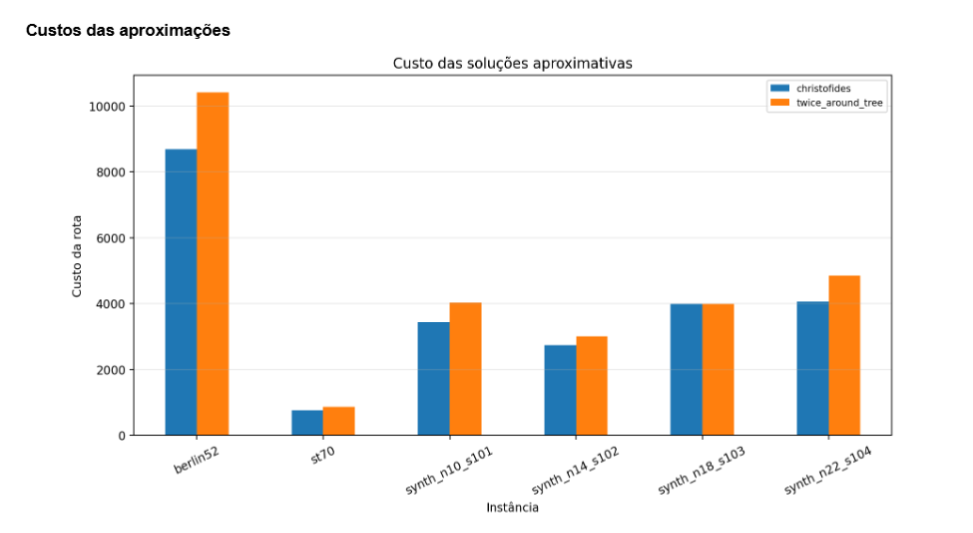
\includegraphics[width=0.75\linewidth]{custoxinstancia.png}
    \caption{Custo das soluções aproximativas para algumas instancias}
    \label{fig:placeholder}
\end{figure}

Neste gráfico, o custo das rotas produzidas pelos algoritmos. O custo corresponde à soma das distâncias percorridas pelo caixeiro-viajante, incluindo o retorno à cidade inicial. Portanto, quanto menor o valor, melhor.

Observamos que Christofides apresentou custos inferiores aos de Twice-around-the-tree em todas as seis instâncias avaliadas. Esse resultado é coerente com sua garantia teórica em que o seu fator 1,5, em comparação ao fator 2 do algoritmo baseado na duplicação da árvore geradora mínima porque Christofides, depois de construir uma árvore geradora mínima, realiza um emparelhamento perfeito de custo mínimo entre os vértices de grau ímpar. Isso evita  duplicar todas as arestas da árvore.





\subsection{Comparação das Estratégias de Inicialização}

A Tabela~\ref{tab:warmstarts} apresenta os resultados
das cinco estratégias de inicialização do
Branch-and-Bound para a instância "Berlin52".

\begin{table}[H]
\centering
\caption{Resultados do Branch-and-Bound por estratégia.}
\label{tab:warmstarts}
\small
\begin{tabular}{lrrrr}
\toprule
Estratégia & Custo & Expandidos & Podados & Tempo (s)\\
\midrule
Cold Start & 8251,76 & 1683555 & 11800748 & 1800,00\\
Nearest Neighbor & 8251,76 & 1655813 & 11521567 & 1800,00\\
Convex Hull & 8105,78 & 1943342 & 13240967 & 1800,00\\
Twice-around-tree & 8251,76 & 1849628 & 13254466 & 1800,00\\
Christofides & 8251,76 & 1842764 & 13179555 & 1800,00\\
\bottomrule
\end{tabular}
\end{table}

Todas as execuções atingiram o limite máximode 30 minutos sem comprovação da otimalidade.
Assim, os custos apresentados correspondem às melhores soluções encontradas durante
o período de execução, não sendo necessariamente os valores ótimos das instâncias.

A estratégia Convex Hull encontrou a menor solução entre as execuções, com custo de 8105,78.
As demais estratégias encontraram soluções com custo de 8251,76.

Apesar de apresentar o menor custo encontrado, Convex Hull também registrou a maior quantidade
de nós expandidos, com 1943342.Esse comportamento indica que a qualidade da solução inicial não determina isoladamente o esforço de busca, sendo necessário considerar também os limites inferiores, a ordem de exploração e a estrutura da árvore de busca.


\subsection{Análise de Tempo e Memória}

Os algoritmos aproximativos apresentaram tempos de execução  inferiores ao
limite estabelecido para o Branch-and-Bound.

Enquanto Twice-around-the-tree e Christofides concluíram suas execuções em frações de segundo
na instância apresentada, todas as execuções do Branch-and-Bound atingiram o limite 


Além da análise do tempo total de execução, foi realizada uma avaliação das principais subrotinas dos algoritmos aproximativos, com o objetivo de identificar quais etapas concentram o custo computacional.

A Tabela~\ref{tab:subrotinas_tsp} apresenta os tempos médios de execução, a participação percentual de cada subrotina no tempo total e o pico de memória registrado.

Os resultados mostram comportamentos distintos entre os algoritmos.

No algoritmo de Christofides, a etapa de emparelhamento perfeito de custo mínimo representa a maior parcela do tempo total. A construção da árvore geradora mínima representa 9,8\%, enquanto as demais operações correspondem a 32,4\%.

Esse resultado evidencia que o matching constitui uma etapa relevante do custo computacional de Christofides. A identificação dos vértices de grau ímpar e o cálculo do emparelhamento perfeito introduzem um processamento adicional em comparação com o Twice-around-the-tree.


A comparação também evidencia a diferença de tempo entre os métodos. O tempo total médio registrado para Christofides foi de 0,0183 segundo, enquanto Twice-around-the-tree apresentou 0,0013 segundo.

Em relação à memória, Christofides apresentou pico de 0,11 MB, enquanto Twice-around-the-tree apresentou 0,06 MB. Esses valores indicam maior consumo de memória registrado para Christofides nas condições avaliadas.

É importante destacar que a participação percentual das subrotinas depende da implementação, das estruturas de dados utilizadas e das características das instâncias.

De modo geral, a análise permite identificar diferentes pontos de atenção para otimização, no Christofides, o emparelhamento representa a principal parcela individual do tempo, enquanto no Twice-around-the-tree a construção da árvore geradora mínima concentra a maior parte do processamento.


\begin{table}[H]
\centering
\caption{Análise de subrotinas: tempo médio, participação percentual e pico de RAM.}
\label{tab:subrotinas_tsp}
\small
\setlength{\tabcolsep}{3pt}
\resizebox{\textwidth}{!}{%
\begin{tabular}{lrrrrrrrr}
\hline
Algoritmo & Total (s) & AGM (s) & AGM (\%) &
Emp. (s) & Emp. (\%) & Outros (s) & Outros (\%) & RAM (MB) \\
\hline
Christofides & 0.0183 & 0.0007 & 9.8\% &
0.0147 & 57.8\% & 0.0029 & 32.4\% & 0.11 \\
Twice-around-tree & 0.0013 & 0.0010 & 72.2\% &
-- & -- & 0.0003 & 27.8\% & 0.06 \\
\hline
\end{tabular}%
}
\end{table}





\subsection{Auditoria com estratégia Best First}

\begin{table}[H]
\centering
\caption{Desempenho comparativo dos algoritmos aproximativos e variantes de Warm-Start no Branch-and-Bound.}
\label{tab:resultados_log}
\resizebox{\textwidth}{!}{%
\begin{tabular}{llrrrrc}
\toprule
\textbf{Instância} & \textbf{Algoritmo / Warm-Start} & \textbf{Custo} & \textbf{Tempo (s)} & \textbf{Nós Exp.} & \textbf{Nós Pod.} & \textbf{Status} \\
\midrule
\multirow{7}{*}{\texttt{berlin52}} 
  & Twice-around-the-tree & 10403,86 & 0,0032 & -- & -- & Aproximado \\
  & Christofides & 8688,45 & 0,0347 & -- & -- & Aproximado \\
  & B\&B (Cold Start) & 22205,62 & 101,1154 & 25537 & 0 & Timeout \\
  & B\&B (Nearest Neighbor) & 8980,92 & 99,7095 & 25537 & 0 & Timeout \\
  & B\&B (Convex Hull) & 8105,78 & 99,7808 & 25537 & 0 & Timeout \\
  & B\&B (Twice-around) & 10403,86 & 99,5696 & 25537 & 0 & Timeout \\
  & B\&B (Christofides) & 8688,45 & 100,9784 & 25537 & 0 & Timeout \\
\midrule
\multirow{7}{*}{\texttt{st70}} 
  & Twice-around-the-tree & 861,77 & 0,0017 & -- & -- & Aproximado \\
  & Christofides & 753,15 & 0,0591 & -- & -- & Aproximado \\
  & B\&B (Cold Start) & 3410,56 & 149,7629 & 17813 & 0 & Timeout \\
  & B\&B (Nearest Neighbor) & 805,53 & 150,1647 & 17813 & 0 & Timeout \\
  & B\&B (Convex Hull) & 707,43 & 150,1491 & 17813 & 0 & Timeout \\
  & B\&B (Twice-around) & 861,77 & 149,1445 & 17813 & 0 & Timeout \\
  & B\&B (Christofides) & 753,15 & 149,2431 & 17813 & 0 & Timeout \\
\midrule
\multirow{7}{*}{\texttt{synth\_n10}} 
  & Twice-around-the-tree & 4032,96 & 0,0010 & -- & -- & Aproximado \\
  & Christofides & 3436,59 & 0,0040 & -- & -- & Aproximado \\
  & B\&B (Cold Start) & \textbf{3376,47} & 1,1888 & 40783 & 26656 & Ótimo \\
  & B\&B (Nearest Neighbor) & \textbf{3376,47} & 1,3606 & 40613 & 26656 & Ótimo \\
  & B\&B (Convex Hull) & \textbf{3376,47} & \textbf{0,8449} & \textbf{14126} & 26657 & Ótimo \\
  & B\&B (Twice-around) & \textbf{3376,47} & 1,1628 & 39663 & 26656 & Ótimo \\
  & B\&B (Christofides) & \textbf{3376,47} & 1,0271 & 17464 & 26656 & Ótimo \\
\midrule
\multirow{7}{*}{\texttt{synth\_n14}} 
  & Twice-around-the-tree & 2998,84 & 0,0007 & -- & -- & Aproximado \\
  & Christofides & 2732,10 & 0,0046 & -- & -- & Aproximado \\
  & B\&B (Cold Start) & 5847,20 & 44,0179 & 284807 & 0 & Timeout \\
  & B\&B (Nearest Neighbor) & 2727,03 & 87,2027 & 671016 & 1161829 & Timeout \\
  & B\&B (Convex Hull) & \textbf{2569,64} & \textbf{134,3986} & \textbf{1307296} & \textbf{3745481} & \textbf{Ótimo} \\
  & B\&B (Twice-around) & 2998,84 & 45,1771 & 291412 & 20811 & Timeout \\
  & B\&B (Christofides) & 2732,10 & 82,5947 & 634528 & 1056357 & Timeout \\
  \midrule
\multirow{7}{*}{\texttt{synth\_n18}} 
  & Twice-around-the-tree & 3989,90 & 0,0007 & -- & -- & Aproximado \\
  & Christofides & 3983,69 & 0,0060 & -- & -- & Aproximado \\
  & B\&B (Cold Start) & \textbf{3427,91} & 8,4512 & 187726 & 165714 & Ótimo \\
  & B\&B (Nearest Neighbor) & \textbf{3427,91} & 7,4982 & 150967 & 165714 & Ótimo \\
  & B\&B (Convex Hull) & \textbf{3427,91} & \textbf{5,5375} & \textbf{22011} & 165715 & Ótimo \\
  & B\&B (Twice-around) & \textbf{3427,91} & 7,7178 & 157384 & 165714 & Ótimo \\
  & B\&B (Christofides) & \textbf{3427,91} & 7,5346 & 155700 & 165714 & Ótimo \\
\bottomrule
\end{tabular}%
}
\end{table}

A tabala abaixo representa um resumo a partir dos resultados experimentais obtidos com a estratégia de busca em profundidade  no algoritmo Branch-and-Bound. 

\begin{table}[htbp]
\centering
\caption{Resumo experimental de custo, tempo, memória e busca no TSP.}
\label{tab:resumo_tsp}
\small
\setlength{\tabcolsep}{3pt}
\resizebox{\textwidth}{!}{%
\begin{tabular}{llrrrrrr}
\hline
Algoritmo & Warm-Start & Custo Méd. & Tempo (s) & RAM (MB) &
Nós Exp. & Heap Máx. & Timeouts \\
\hline
B\&B & Christofides & 3730.81 & 375.6166 & 96.28 & 619322.3 & 285818.5 & 5 \\
B\&B & Cold Start & 5339.37 & 344.3088 & 100.84 & 641125.0 & 298951.7 & 5 \\
B\&B & Convex Hull & 3644.85 & 347.0085 & 69.03 & 500030.4 & 202175.9 & 4 \\
B\&B & Nearest Neighbor & 3759.41 & 347.3195 & 99.97 & 654734.2 & 295872.7 & 5 \\
B\&B & Twice-around-tree & 3906.13 & 344.3570 & 99.99 & 653217.5 & 296328.2 & 5 \\
Christofides & -- & 3981.20 & 0.0183 & 0.11 & -- & -- & 0 \\
Twice-around-tree & -- & 4591.02 & 0.0013 & 0.06 & -- & -- & 0 \\
\hline
\end{tabular}%
}
\end{table}





	\section{Conclusão}
	\label{sec_conclusao}
	
	Este trabalho apresentou a implementação e a avaliação experimental de
algoritmos  exatos e aproximativos para o Problema do Caixeiro Viajante.
Foram estudados o Branch-and-Bound, o Twice-around-the-tree e o al-
goritmo de Christofides, além de cinco estratégias de inicialização para o
método exato.
Nos experimentos realizados, Christofides apresentou custos inferiores aos
de Twice-around-the-tree nas  instâncias avaliadas. Em contrapartida, o
Twice-around-the-tree apresentou menor tempo de execução, comportamento
compatível com a ausência da etapa adicional de emparelhamento perfeito.
A análise das estratégias de inicialização do Branch-and-Bound mostrou
que Convex Hull apresentou resultados expressivos nas instâncias sintéticas
concluídas, reduzindo a quantidade de nós expandidos em comparação com
as demais estratégias.
Nas instâncias maiores, as execuções do Branch-and-Bound atin-
giram o limite de tempo. Esses resultados
evidenciam a dificuldade de utilizar a busca exata em instâncias maiores,
mesmo quando mecanismos de poda são empregados.
A análise das características geométricas permitiu descrever diferenças
entre as instâncias. Como continuidade do trabalho, destacam-se a ampliação do conjunto de
instâncias, a realização de novas execuções controladas, a comparação  entre Best-First e DFS, o ajuste de curvas empíricas de complexidade
e o aprofundamento da análise de sensibilidade das características geométricas

  
	
\end{document}
